The first step in the design process is to understand the domain of the API\@.
This helps identify required input parameters, return values, and types expressed in the domain language.
It is also important to capture possible API evolution in the future so that the modeled API is flexible enough
to support it without drastic changes and breaking backward compatibility.

There are three types of IGMPv2 messages: Membership Query, Membership Report, and Leave Group message.
All message types follow the same format of the packet header but with different values in the fields.
The structure of the IGMPv2 packet is depicted in Figure~\ref{fig:igmp_packet}.

\begin{figure}[!htb]
\centering
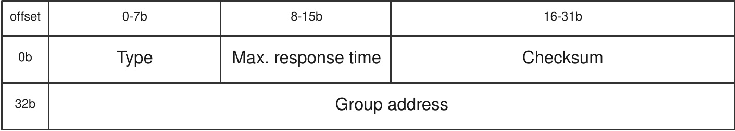
\includegraphics[width=1.0
\textwidth]{igmp_packet}
\caption{Structure of the IGMPv2 packet}
\label{fig:igmp_packet}
\end{figure}

From the perspective of API design, there are the following key differences between constructed types of packets:

\begin{enumerate}
    \item Membership Query:
    The type field is set to the \textit{0x11} value.
    Both maximum response time and group address can have a non-zero value.
    In the case of a General Query, the group address is set to the \textit{0.0.0.0} value
    (all multicast groups are queried in the broadcast domain).
    In the case of a Group-Specific Query, the group address should contain a valid multicast address
    that is queried by the router.
    \item Membership Report:
    The type field is set to the \textit{0x12} value.
    Maximum response time is always set to \textit{0} (unused).
    The group address should contain a valid multicast address reported by the client.
    \item Leave Group:
    The type field is set to the \textit{0x17} value.
    Maximum response time is always set to \textit{0} (unused).
    The group address should contain a valid multicast address that the client wants to leave.
\end{enumerate}

The following list summarizes the findings from the domain analysis that we have to keep in mind during
the design process:

\begin{itemize}
    \item
    There are three types of IGMPv2 messages that differ in the constant values of the fields.
    Serialization logic, which will be implemented as the business logic, is common for all types of messages.
    \item
    There are two configurable parameters (aside from the type of message) that the client should be able to specify
    on the input: maximum response time and group address.
    However, there are some constraints on the values of these parameters based on the type of the IGMPv2 message
    (for example, Leave Group message maximum response time is always set to 0) and field length (number of bytes).
    \item
    The API should not define any return type since serialized data will be written to the output stream
    (for example, backed by a network socket) that is passed as the input parameter.
    \item
    In the future, the client may require support for IGMPv1 and IGMPv3 protocols.
    Especially IGMPv3 protocol specifies additional fields in the packet header that are not present
    in the IGMPv2 protocol.
    There is also an open room for possible support of the IPv6 flavor of the IGMP protocol
    - Multicast Listener Discovery (MLD) that is implemented by the Internet Group Management Protocol (IGMP).
\end{itemize}
